

\section{预备知识}\label{sec:pre}


图表示学习在过去几十年中一直是一个被广泛研究的方向。如图~\ref{fig:pre1} 所示，这一研究脉络经历了从浅层嵌入方法到监督式图神经网络的发展，并进一步从“预训练-微调”范式演进到新兴的“提示（prompt）”范式。在本节中，我们将概述本文所使用的基本符号记号，回顾图表示学习的历史发展，介绍预训练与微调范式，并梳理基于提示的学习范式的演化。更为重要的是，我们将提出一个聚焦于\textbf{灵活性（flexibility）}与\textbf{表达能力（expressiveness）}的新视角，用以阐明为何提示为突破既有图表示学习方法的局限提供了有前景的解决思路。



\subsection{符号记号}\label{subsec:notation}

设一个图实例表示为 $\mathcal{G} = \{ \mathcal{V}, \mathcal{E} \}$，其中 $\mathcal{V} = \{ v_1,v_2, \ldots, v_N \}$ 表示包含 $N$ 个节点的节点集合。边集合 $\mathcal{E} \in \mathcal{V} \times \mathcal{V}$ 描述节点之间的连接关系。每个节点 $v_i$ 关联一个特征向量，记为 $\textbf{x}_i \in \mathbb{R}^D$。为刻画图的连通性，我们使用邻接矩阵 $\textbf{A} \in \{0,1\}^{N \times N}$，其中当且仅当边 $(v_i,v_j) \in \mathcal{E}$ 时，$\textbf{A}_{ij} = 1$。



\subsection{图表示学习}

过去几十年见证了图表示学习技术的显著发展。相关方法大体可分为两条主线：浅层嵌入方法与深层图神经网络（GNN）。浅层嵌入方法的核心是将节点映射到低维、可学习的嵌入空间，从而便于在各类下游任务中使用，其代表包括 node2vec~\cite{grover2016node2vec} 与 DeepWalk~\cite{perozzi2014deepwalk}。与之相对，深层 GNN 通常将输入节点特征视为常量，并针对特定任务优化深层图模型参数，从而获得更强的表示能力，例如图卷积网络（GCN）~\cite{niepert2016learning} 与 GraphSAGE~\cite{hamilton2017inductive} 等方法。



浅层嵌入方法将输入节点特征视作可学习参数，旨在以保留原始网络相似性结构的方式对节点进行编码。

根据节点相似性的定义，这类方法可进一步分为基于分解的技术~\cite{% belkin2001laplacian,
% ahmed2013distributed,
% cao2015grarep,
ou2016asymmetric, zhang2019prone} 与基于随机游走的技术~\cite{grover2016node2vec, perozzi2014deepwalk, wang2019hyperbolic, wang2022common}。

尽管浅层嵌入方法在不同下游任务中具有较高的灵活性，但其受限于无法为训练阶段未出现的节点生成嵌入表示；此外，这类方法通常难以有效融合节点属性特征。因此，研究者提出了更“深”的方法，尤其是基于图神经网络的方案，以弥补上述不足。



多数深层 GNN 遵循消息传递（message-passing）范式，并采用更复杂的编码器，从而在图表示方面具有更强的表达能力。典型的网络结构是卷积式图神经网络（ConvGNNs），其包含谱域方法~\cite{defferrard2016convolutional,he2021bernnet}

以及空间域方法~\cite{% atwood2016diffusionconvolutional,
niepert2016learning, hamilton2017inductive,
% gao2018largescale,
velickovic2018graph, shi2021masked, xu2018how}。

尽管这些方法在多种图应用中表现出色，但它们对任务特定监督信号的依赖限制了其适应性与泛化能力，尤其是在标注数据稀缺的任务场景下尤为明显。



综上所述，浅层嵌入方法具有更强的灵活性，能够较直接地保留网络结构与节点内容以支持图分析任务；但其表达能力不足，且难以充分表征额外的节点属性。相反，GNN 能够学习更具表达力的图表示，但通常需要任务特定的训练数据，因而迁移性受限。因此，我们需要一种能够同时兼顾表达能力与灵活性的图学习机制，这也推动了“预训练-微调”范式的发展。



\begin{figure}[!t]

    \centering

    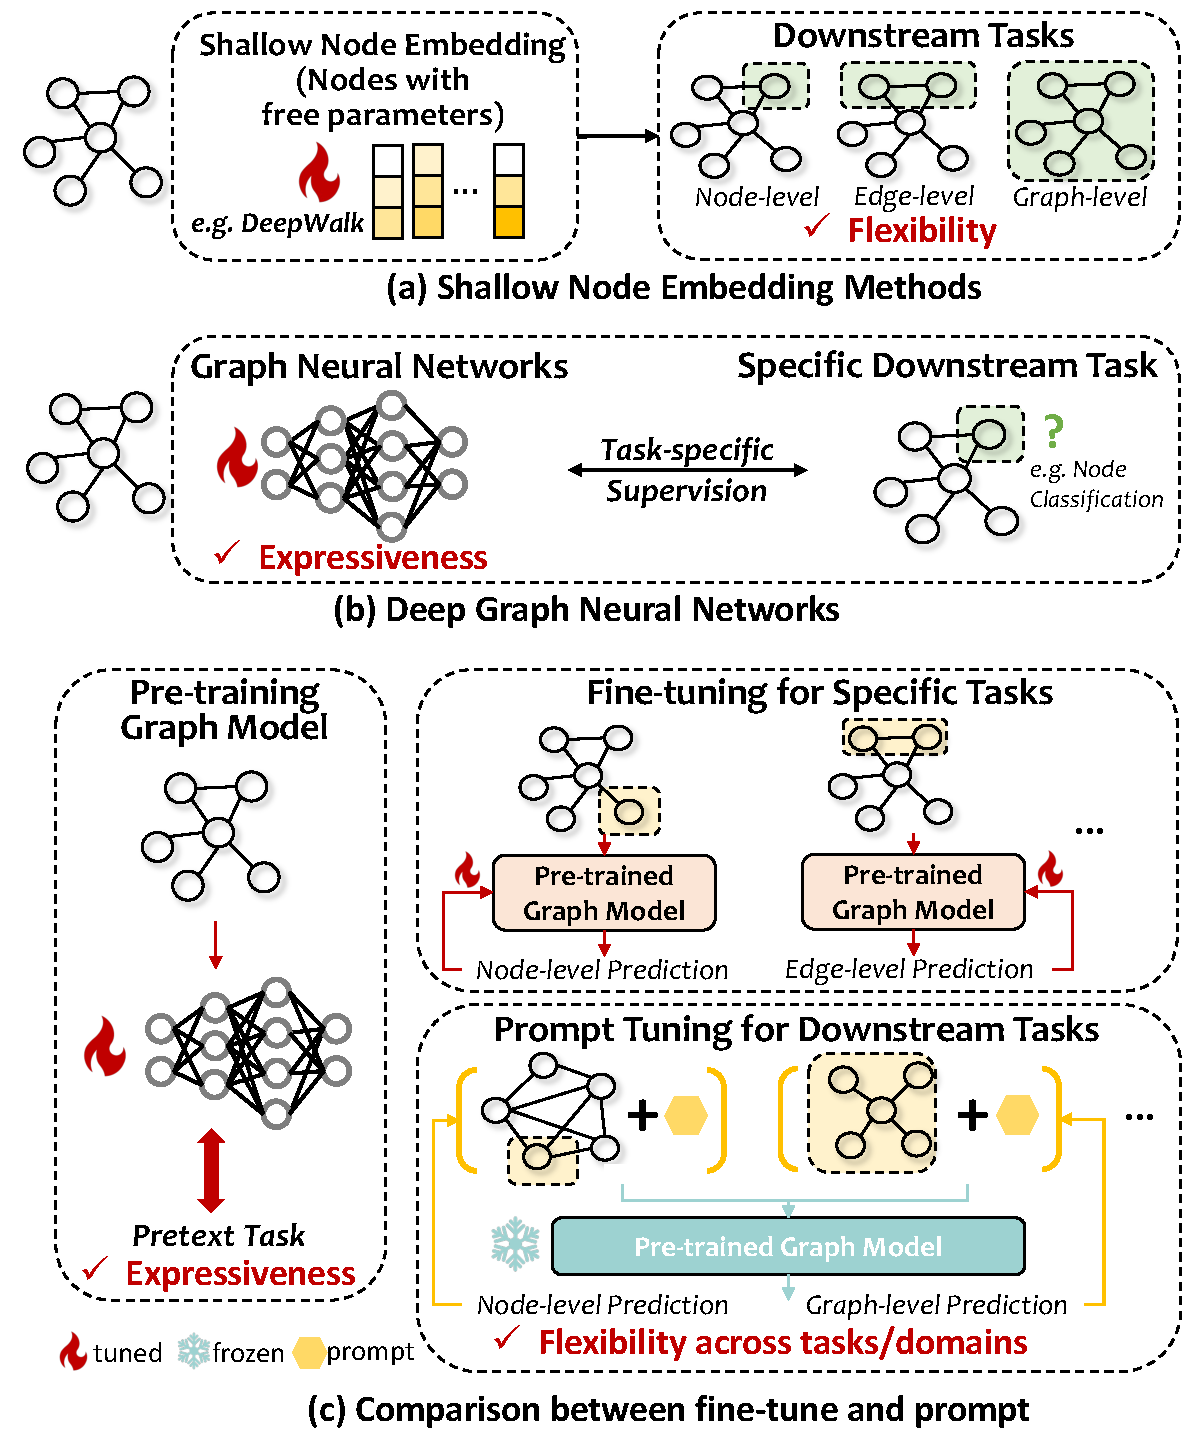
\includegraphics[width=0.49\textwidth]{pic/WhyPrompt2.pdf}

    \caption{我们关于提示在灵活性与表达能力上的视角。（a）浅层节点嵌入方法在不同下游任务间具有灵活性，但牺牲了表达能力。（b）GNN 具备较强表达能力，但需要任务特定监督且将节点特征视为常量，从而限制其灵活性。（c）提示机制提供一种折中路径，可同时兼顾灵活性与表达能力。}

    \label{fig:pre1}

\end{figure}


\subsection{预训练与微调}

为应对 GNN 在标注数据不足与泛化方面的挑战，源自自然语言处理（NLP）社区并发展成熟的“预训练-微调”范式已被广泛引入图表示学习。该范式通常先在大规模图数据（有标注或无标注）上对模型进行预训练，随后在多样化下游任务上对模型参数进行微调。这一两阶段流程能够改进模型初始化，使优化更易落入更“宽”的最优区域，从而相较于从零训练获得更好的泛化性能。常见的图预训练方案包括图自编码器（GAEs）~\cite{% kipf2016variational,
wang2017mgae}、掩码组件建模（MCM）~\cite{hu2020strategies, rong2020selfsupervised}、图对比学习（GCL）~\cite{velickovic2019deep, sun2020infograph} 等。在第~\ref{sec:pretrain_method} 节中，我们将对预训练与微调方法进行更为细致的讨论，以给出更全面的图景。



\subsection{提示学习简史}\label{subsec:his_prompt}


随着模型参数规模不断增大，传统的\emph{预训练-微调}流程正在演进为一种新的范式：\emph{预训练、提示与预测}~\cite{liu2023pretrain}。在该范式中，不再需要针对每个下游任务手工适配并更新预训练模型参数；相反，借助提示将下游任务重述为与预训练阶段相似的问题形式。


NLP 中的提示具有多种形态，包括完形填空式提示（cloze prompts）

% ~\cite{

% % cui2021templatebased,

% petroni2019language}

（用于掩码语言模型中对文本片段进行补全），以及前缀提示（prefix prompts）~\cite{lester2021power,li2021prefixtuning}（在自回归语言模型中将输入文本置于答案槽之前）。一些研究基于人类先验手工设计模板~\cite{% petroni2019language,
brown2020language,schick2021fewshot,schick2021it}，另一些研究则探索自动化模板学习，包括在离散空间中搜索模板~\cite{jiang2020how, haviv2021bertese, shin2020autoprompt,gao2021making}，或直接在嵌入空间中进行提示~\cite{li2021prefixtuning, lester2021power,tsimpoukelli2021multimodal,qin2021learning}。


该范式使得单个预训练模型能够以（近）无监督的方式处理大量下游任务，这一点已被大规模语言模型广泛验证。受此启发，将提示技术应用于图任务背景之下，已成为当前一个活跃的探索方向。



\subsection{为何使用提示？基于灵活性与表达能力的新视角}\label{subsec:why_prompt}



为何提示学习在图领域具有潜力？多数相关工作常用的观点是：提示可以将下游任务重述为预训练任务，从而弥合二者之间的差距。该观点有其合理性，但仍不足以揭示提示与传统微调之间的内在差异。举例而言，从相似的表述角度看，“预训练-微调”也可被理解为用微调将预训练任务重述为下游任务——似乎两条技术路线都在解决同一类问题。那么，为什么提示往往会成为更优选择？



为回答这一问题，我们提出一个新的分析视角，以更清晰地刻画提示与微调之间的差异。正如前文所述，现有图表示学习方法难以在表达能力与灵活性之间取得令人满意的折衷。浅层图嵌入方法具有较强灵活性，可适用于多种下游任务；但由于参数化能力有限且难以融合原始节点特征，其表达能力受限。以 DeepWalk 为例，浅层图方法往往将节点表示视作自由参数，因此每个节点可以相对独立地学习其表示，表现出很强的灵活性。但受梯度学习机制所限，它们通常难以在后续引入更复杂的深层网络，从而可能损失一部分表达能力。事实上，已有不少更先进的工作会将 DeepWalk 学到的节点表示作为输入特征，叠加深层图网络，以利用其跨任务的通用性。另一方面，基于 GNN 的方法将节点嵌入视为常量特征，并尝试学习一个强大的网络将节点特征映射到特定任务上，因此具有更强表达能力。然而，这种学习到的特征变换模式会统一施加于所有节点，意味着模型无法将每个节点嵌入视为自由参数，从而难以获得与浅层方法同等的灵活性。当存在多个任务时，通常需要训练同一 GNN 的不同版本，这在灵活性上不如浅层方法。



基于上述分析可知，传统微调的目标在于利用预训练图模型进一步提升新任务上的表达能力，但难以兼顾节点层面的灵活性。与微调不同，图提示通常包含若干带有自由参数的提示 token，这一点与浅层图方法更为相似。同时，原始图中的节点在 GNN 模型中通常具有常量特征。通过将提示图插入到原始图中，组合后的图同时包含“常量特征节点”与“自由参数 token”。其中，自由参数 token 可以被高效地调优，从而保留节点层面的灵活性；而组合图则被送入冻结的预训练 GNN，以利用深层图模型所具备的强表达能力。



因此，本文认为提示机制为克服现有图表示学习方法的局限提供了一条有前景的路径，即在\textbf{灵活性}与\textbf{表达能力}之间实现有效平衡。预训练 GNN 本身蕴含结构与语义层面的知识，能够提供所需的表达能力；引入提示后，我们能够以更高效的方式将强大的预训练模型迁移到不同领域的多样下游任务中。这通过将下游任务的输入/目标形式与预训练任务的形式对齐来实现，从而即使在监督信号极少的情况下，也能充分发挥预训练模型的潜力。尽管微调机制同样能够促进预训练图模型的领域或任务适配，但它往往需要较多标注信息，并且通常需要对预训练模型进行耗时的再次训练。相比之下，提示机制在灵活性与效率上更具优势。
